\label{sec:detectfalseshare}

This section first describes the basic idea of detecting false sharing. 

\subsection{Basic Idea}
\label{sec:detectionidea}

There is a false sharing problem when two threads simultaneously access independent data in the same cache line. False sharing does not necessarily cause performance problems. It can greatly degrade performance only when those accesses, caused by threads running on different cores with separate cache, actually cause a big number of cache invalidations. This is our \textbf{basic observation}. 

However, it is hard to know where a thread is located in the user space. Moreover, it is unnecessary to know this relationship since the relationship between threads and cores can be changed from one execution to the other. Thus, we make the following \textbf{assumptions}. First, we conservatively assume that all threads are running on different cores, with separate caches. Thus we can report the worst-case results caused by false sharing problems. In order to avoid expensive cache simulation, which can be affected by cache hierarchy, cache capacity and cache eviction rule, we further assume that the data is never evicted from its private cache by cache eviction, with infinite cache. This second assumption allows us to predict the cache invalidations based on memory accesses only, no need to think about cache eviction.   

Based on our basic observation, detecting false sharing problems turns into locating cache lines with a big number of cache invalidations. Cache invalidations are invoked by cache coherence protocol, the protocol used to ensure the coherence of data in the multiple-processor system. Based on our assumptions, there is a cache invalidation if a processor writes a cache line after another thread's access on the same cache line. Because the last thread accessing this cache line creates a copy of the same cache line on its running core's private cache (first assumption) and  holds this copy(second assumption), this write operation definitely cause a cache invalidation before or after this write operation, depending on different cache coherence protocols. 

\begin{figure}[!t]
\centering
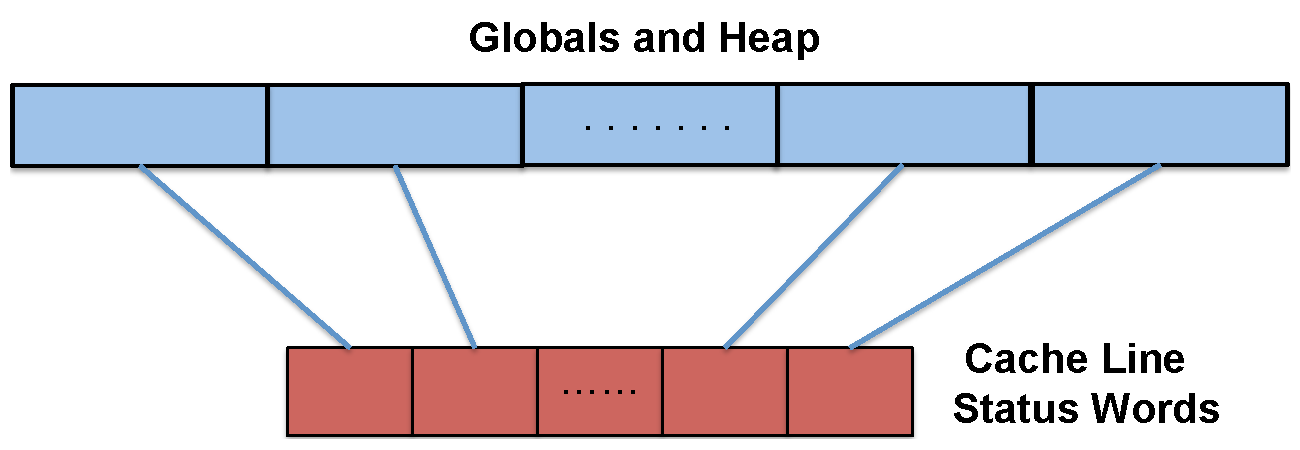
\includegraphics[width=5in]{fig/cachelinestatuswords}
\caption{
To detect false sharing, each cache line of the globals and heap maintains a cache line status word, which is updated on each tracked memory access. \label{fig:cachelinestatusword}}
\end{figure}


To locate cache lines with a big number of cache invalidation, we maintain a cache line status word for each cache line in the globals and heap, shown in Figure~\ref{fig:cachelinestatusword}. We share the similar mechanism as another concurrent work of Zhao et.al. ~\cite{qinzhao}. However, the detailed implementation is totally different. Zhao et.al. utilize the detailed ownership bitmap and last thread bitmap to precisely track the cache invalidation, which can even track how many cache invalidations may happen in a write operation. However, their design can not easily scale to more than 32 threads, requiring more memory overhead caused by more bits and more checking performance overhead. Also, their approach miss one important factor - how many cache invalidations happening on a specific cache line. Without this information, it is impossible to pinpoint false sharing problems that can cause performance problems.   
Our approach overcomes all these shortcomings, by only tracking the last thread index and the number of cache invalidations. Thus, we can rank the seriousness of false sharing problems based on the number of cache invalidations. 

\subsubsection{Accurate Detection}
\label{sec:accuratedetect}

Accurate detection implies that we only report those false sharing problems that can cause performance problems. 

First, we only report those problems that can cause performance problems. This has been resolved by only reporting false sharing with a big number of cache invalidations. 

Second, this also implies that we should be able to differentiate false sharing from true sharing. As we all know, true sharing also can cause cache invalidations, which is the essence to have coherence protocol. In order to differentiate false sharing with true sharing, we further  track word-level access information for those cache lines involved in false sharing: how many reads or writes to each word by which thread. When a word is accessed by multiple threads, we mark the origin of this word as a shared access and do not track threads for further accesses to it. This information lets us accurately distinguish false sharing from true sharing in the reporting phase. It also helps diagnose where actual false sharing occurs when there are multiple fields or multiple objects in the same cache line, as this can greatly reduce the manual effort required to fix the false sharing problems.
  
Third, we should avoid pseudo false sharing (false positives) caused by memory reuses.  We update recording information at memory de-allocations for those objects without false sharing problems; heap objects involved in false sharing are never reused so that they can be reported in the end or on demand. 

\subsubsection{Precise Detection}
\label{sec:precisedetect}

Precise detection implies that we can precisely point out where the problem is. Thus, programmers can leverage on that to identify and correct false sharing. 

We identify globals directly by using debug information that associates the address with the name of the global. In order to precisely report the origins of heap objects with false sharing problems, we collect callsite information for each heap object by intercepting memory allocations and deallocations, and report to users about the origins of false sharing objects. 

Also, we present the word-level accesses information to users so that the exact variables or fields that cause performance problems can be determined precisely. 

\subsubsection{Flexible Reporting}
\label{sec:flexiblereport}

We provide two different ways to report those false sharing problems. Normally, we can report those false sharing problems in the end of a program. However, this way does not work for those long-running applications. Thus, we provide a on-demand way of reporting. User can send a specified signal to a corresponding applications. By intercepting those signals, we can report false sharing problems on demand. 

In order to report false sharing problems, we scan cache line status words of the globals and heaps and only report those false sharing problems that can possibly cause performance problems, based on a pre-defined threshold on the number of cache invalidations.  

\subsection{Detailed Implementations}

\label{sec:sheriffdetect}
We provide a tool, \SheriffDetect{}, to detect false sharing problems based on the \sheriff{} framework. The basic idea of \SheriffDetect{} is discussed in Section~\ref{sec:detectfalseshare}. More details is discussed in the following. 

\subsubsection{Tracking Memory Accesses}
\label{sec:memoryaccesses}

\begin{figure*}[!t]
\centering
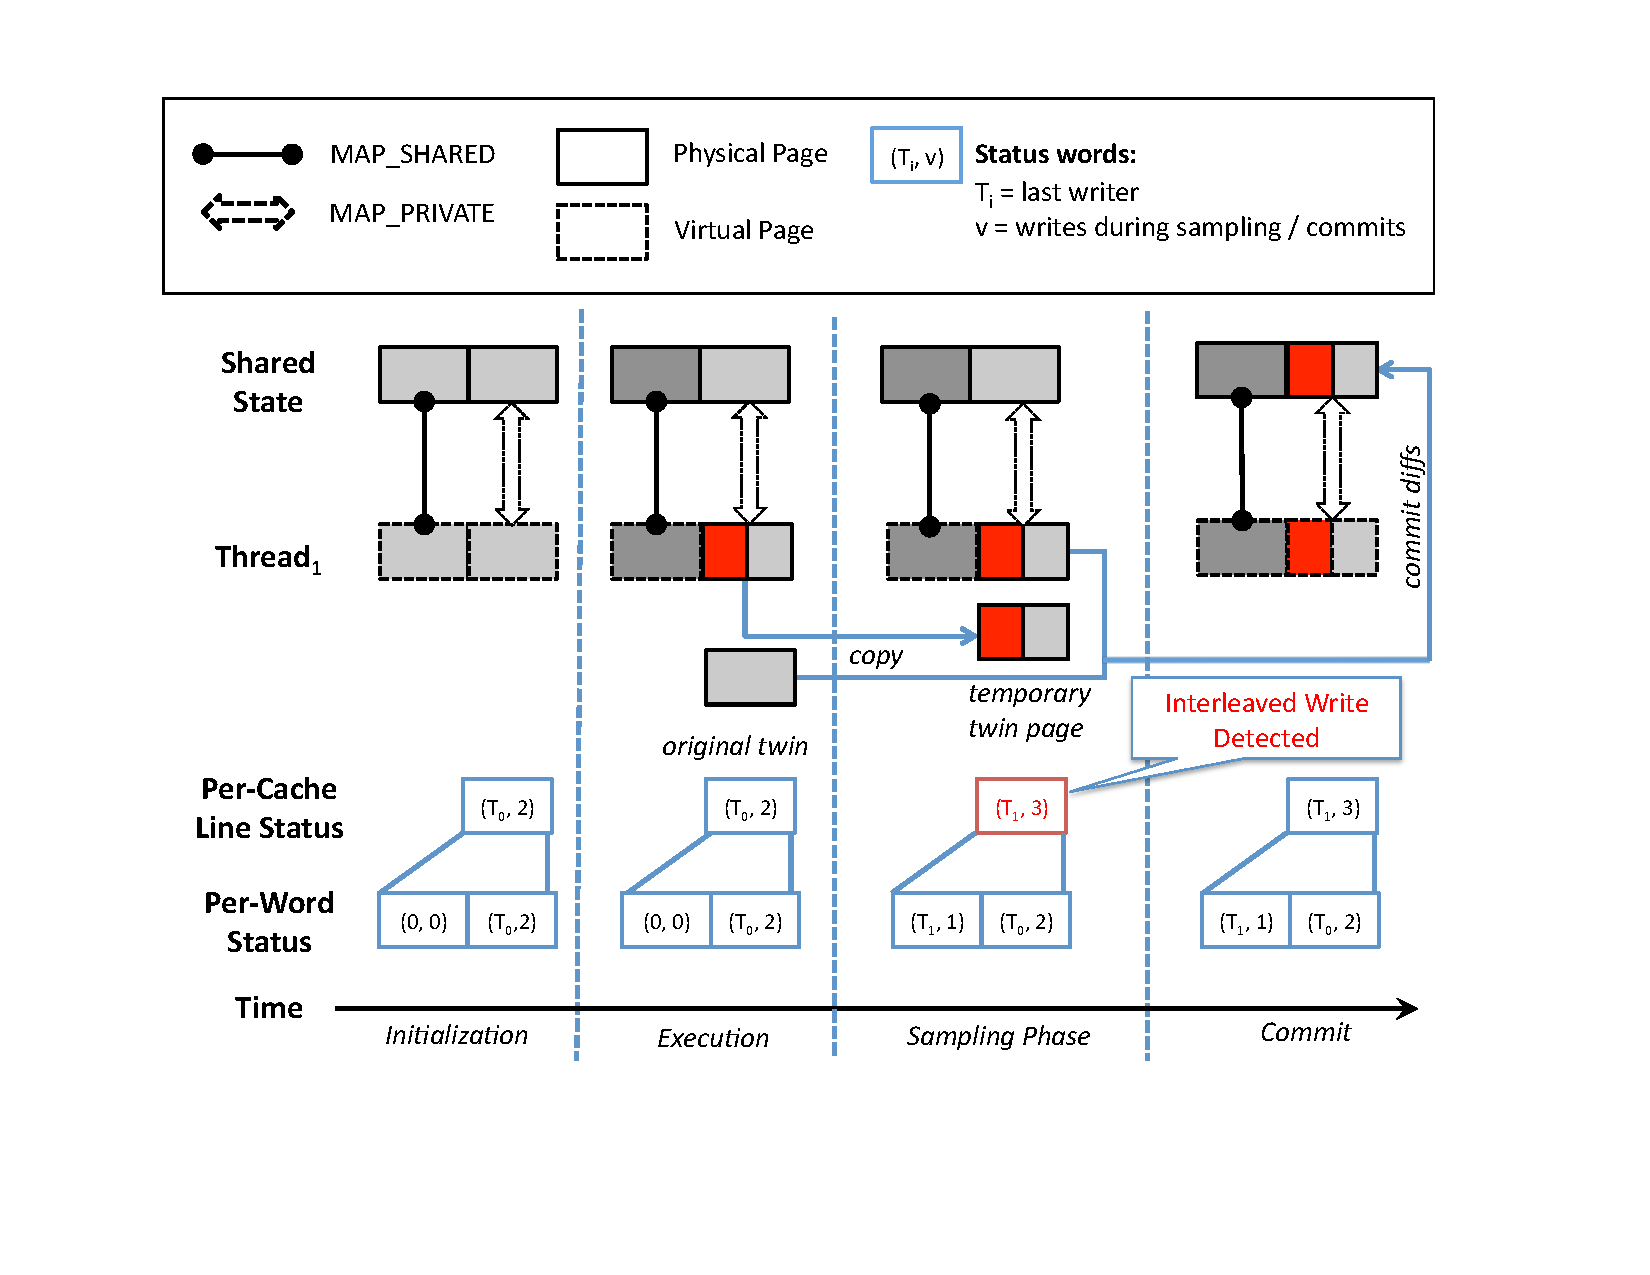
\includegraphics[width=5in]{sheriff/figure/sheriffdetective.pdf}
\caption{
Overview of \SheriffDetect{}’s operation. \SheriffDetect{} extends \Sheriff{} with sampling, per-cacheline status arrays, and per-word status arrays. For clarity of
exposition, the diagram depicts just one cache line per page and two words per cache line.\label{fig:sheriffdetect}}
\end{figure*}

In order to track cache invalidations, we have to track memory accesses of different threads. When there is a memory access, we can check against its corresponding cache line status word to find out whether this memory access causes a cache invalidation or not. \SheriffDetect{} can only track memory writes so that it can only detect write-write false sharing problems. 

\sheriff{} framework provides a strong isolation of different threads' execution and only commits those changes of different threads to the shared mapping in the end of an transaction, by comparing a ``working'' page against its ``twin'' page as described in Section~\ref{sec:sherifftransaction}.
This implies that \sheriff{} is able to find those memory writes at synchronization points. 

However, if a transaction is long-running, finding those memory changes at the end of a transaction is not efficient to find those false sharing problems happening in the middle of a transaction. Actually, the \texttt{linear\_regression} benchmark (described in Section~\ref{sec:evaluation}), degrading the performance by more than $10\times$ because of its false sharing problem, only has a single transaction per thread. 

In order to detect memory accesses in the middle of an transaction, \SheriffDetect{} employs a sampling mechanism using the timer mechanism. When the timer is expired, \SheriffDetect{} tracks memory writes in the current period using the twinning and diffing mechanism. The detailed mechanism is described in Figure~\ref{fig:sheriffdetect}. 

To do this, \SheriffDetect{} also creates a ``temporary twin'' page for every page that have been accessed when the sampling timer is expired. Because these ``temporary twin'' pages are thread-private, we can create and update these pages in the timer handler by simply copying from their corresponding ``working'' pages. The difference between a ``working'' page and its ``temporary'' page implies at least one memory write in this sampling period. Currently, \SheriffDetect{} samples memory accesses of each thread at every 10 microsecond. The tradeoff between sampling period and performance is also discussed in Section~\ref{}. 

\subsubsection{Tracking Cache Invalidations}
\label{sec:invalidation}
As the discussion in Section~\ref{sec:detectionidea}, \SheriffDetect{} tracks and reports those cache lines with a big number of cache invalidations, where they are considered to cause serious performance problems. 

In order to track cache invalidations, \SheriffDetect{} introduces a cache line status word for every cache line of the globals and heap, showed in Figure~\ref{fig:cachelinestatusword}.  Every cache line status word contains two fields, the last thread writing to this cache line and the number of cache invalidations of this cache line. 
Every time, when \SheriffDetect{} detects a memory write, either at the end of transactions or in the sampling timer handler,  it updates these two fields correspondingly. Based on the assumptions described in Section~\ref{sec:detectionidea}, \SheriffDetect{} increments the number of cache invalidations when there is a write from a different thread. To avoid using lock, \SheriffDetect{} updates those counters using atomic primitives. 

\subsection{Optimizations}

\SheriffDetect{} also employs the following optimizations in order to reduce the performance overhead. 

\paragraph{Getting Callsite Information.}
\SheriffDetect{} intercepts memory allocation operations for collecting callsites for every heap object. To reduce the performance overhead, \SheriffDetect{} do not use the bracktrace(), but identify the callsite by analyzing return or frame address using GCC extensions. However, this can not work on applications without debugging information. 

\paragraph{Reducing timer overhead.}
As explained in Section~\ref{sec:memoryaccesses}, \SheriffDetect{} uses sampling to track cache invalidations. To reduce the impact of timer interrupts, \SheriffDetect{} activates sampling only when the average transaction time is larger than a threshold time (currently 10 milliseconds). \SheriffDetect{} uses an exponential moving average to track average transaction times ($\alpha = 0.9$). This optimization does not significantly reduce the possibility of finding false sharing since \SheriffDetect{}'s goal  is to find an object with a large amount of interleaved writes from different threads.

\paragraph{Sampling to find shared pages.} 
To reduce this overhead, \SheriffDetect{} leverages a
simple insight: if two threads can falsely share a cache line,
then they must simultaneously access the page containing
that cache line. \SheriffDetect{} relies on page protection to determine whether pages are shared or not. When one application has a large number of transactions or page touches, the protection overhead to gather this sharing information can dominate running time.

\SheriffDetect{} reduces overhead by using sampling to detect shared pages. If objects on a page are frequently falsely shared, the page itself must also be frequently shared, so even relatively infrequent sampling will eventually detect this sharing.  \SheriffDetect{} currently samples the first 50 out of every 1,000 periods (one period equals one transaction or one sampling interval). At the beginning of each sampled period, all memory pages are made read-only so that any
writes to each page will be detected. Upon finding a page is
shared, \SheriffDetect{} will track any false sharing inside it. \SheriffDetect{} only updates the shared status of pages during sampled periods and at commit points. During unsampled periods, pages whose sharing status is unknown impose no protection overhead.

\subsection{Limitation}
\label{discussion:faultofdetect}

Unlike previous tools, \SheriffDetect{} has no false positives, differentiates true sharing from false sharing, and avoid false positives caused by the reuse of heap objects.
\SheriffDetect{} can under-report false sharing instances in the following situations:

\paragraph{Single writer.}
False sharing usually involves updates from multiple threads, but it can also arise when there is exactly one thread writing to part of a cache line while other threads read from it. Because its detection algorithm depends on at least one differing update (that is, at least two writes of distinct values), \SheriffDetect{} cannot detect this kind of false sharing (though \sheriffprotect{} eliminates it; see Section~\ref{sec:patrol}).

\paragraph{Heap-induced false sharing.}  
\sheriff{} replaces the standard memory allocator with one that, like the Hoard allocator, avoids most heap-induced false sharing. \sheriff{}'s memory allocator (like Hoard), carves memory into page-sized chunks; each thread allocates
from its own set of chunks, and the allocator never splits cache lines across threads. Because \SheriffDetect{} uses the same allocator, it cannot detect false sharing that would be caused by the standard memory allocator. Since it is straightforward to deploy Hoard or a similar allocator to avoid heap-induced false sharing, this limitation is not a problem in practice.

\paragraph{Misses due to sampling.}  Since it uses sampling to
  capture continuous writes from different threads, \SheriffDetect{} can miss writes that occur in the middle of sampling intervals. We hypothesize that false sharing instances that affect performance are unlikely to perform frequent writes exclusively during that time, and so are unlikely to be missed.
